 \section{Annexes}
  \subsection{Test de couverture par sommets qui n'aboutit pas...\label{an1}}
  Couverture par sommets arrétée après plus de 15 minutes: image
  \ref{lourd} page \pageref{lourd}. Même après plus de 30 minutes le
  résultat est le même mais nous n'avons pas d'image pour celui-là car
  nous avons dû redemarrer le pc... En effet on voit la memoire se
  remplir jusqu'à être pleine.

  \begin{figure}[!ht]
   \begin{center}
    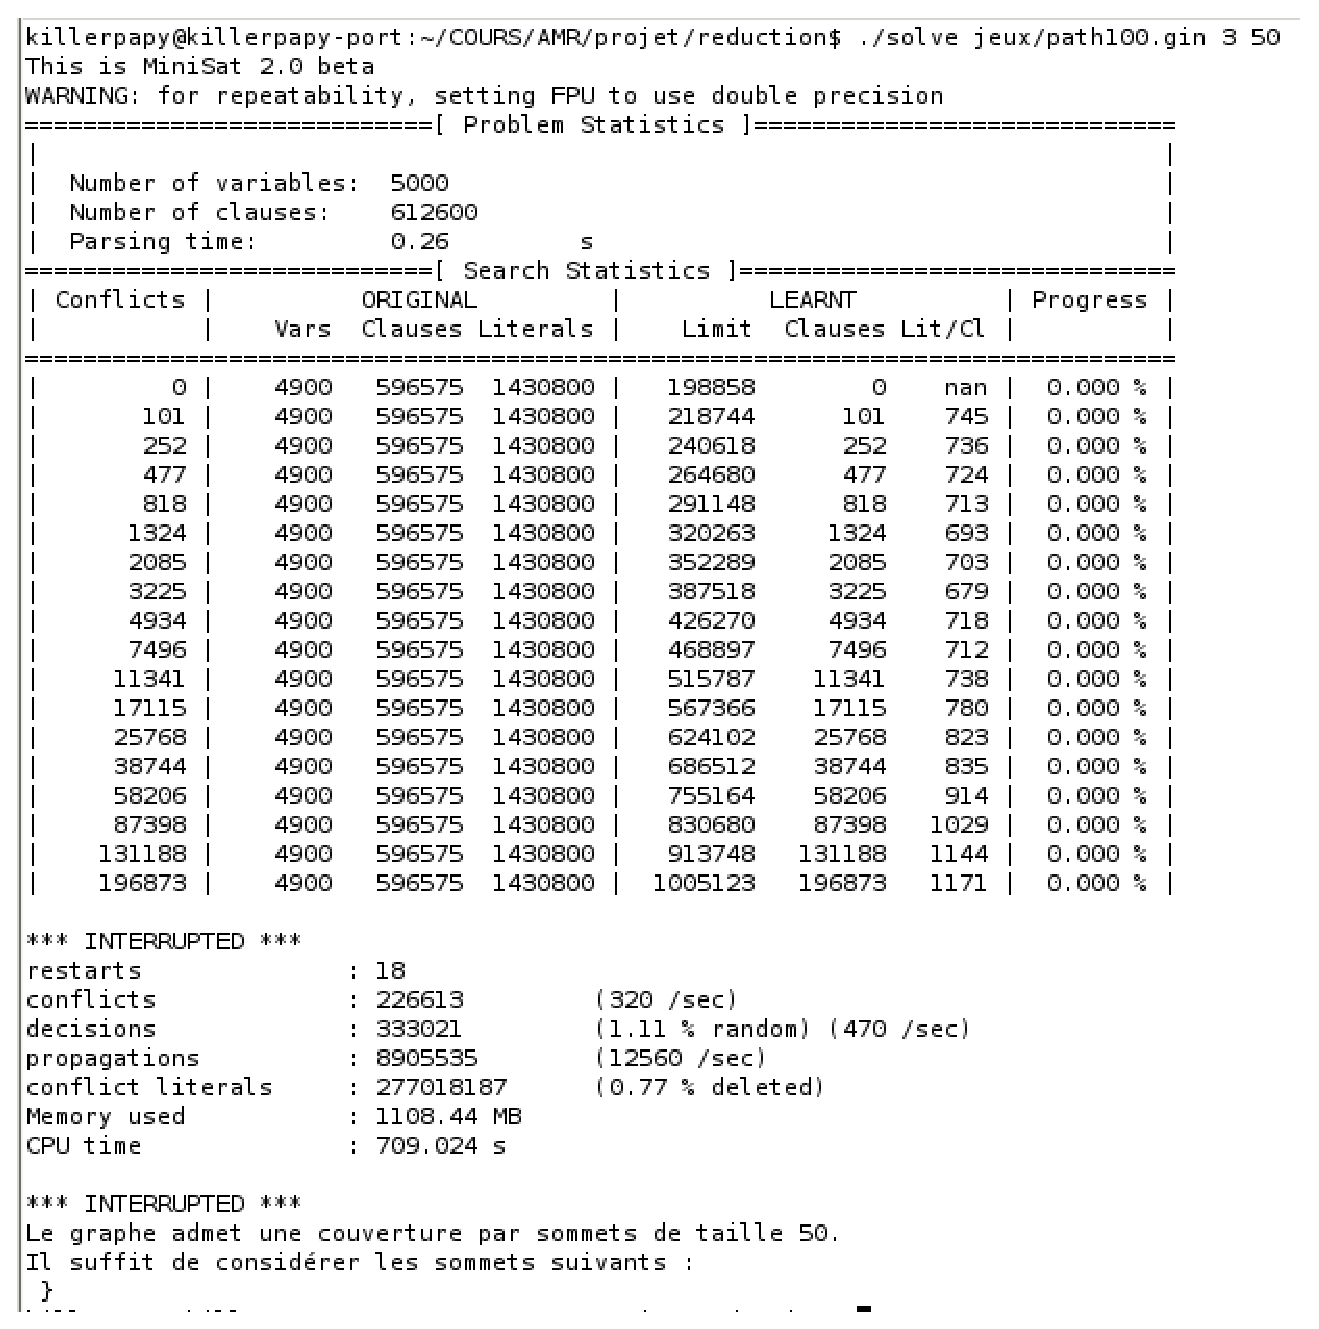
\includegraphics[width=12cm]{images/couv100.eps}
    \caption{\emph{Couverture par sommets} de taille 50 dans un chemin
    de taille 100.\label{lourd}}
   \end{center}
  \end{figure}

  \newpage

  \subsection{Test de KCol sur un petit graphe\label{an2}}
  \emph{3-Col} sur graphe \ref{graphe} page \pageref{graphe} de petite
  taille.
  \begin{figure}[!ht]
   \begin{center}
    \includegraphics[height=6cm]{images/jeurap.ps}
    \caption{Exemple de graphe à 4 sommets.\label{graphe}}
   \end{center}
  \end{figure}
  
  \begin{figure}[!ht]
   \begin{center}
    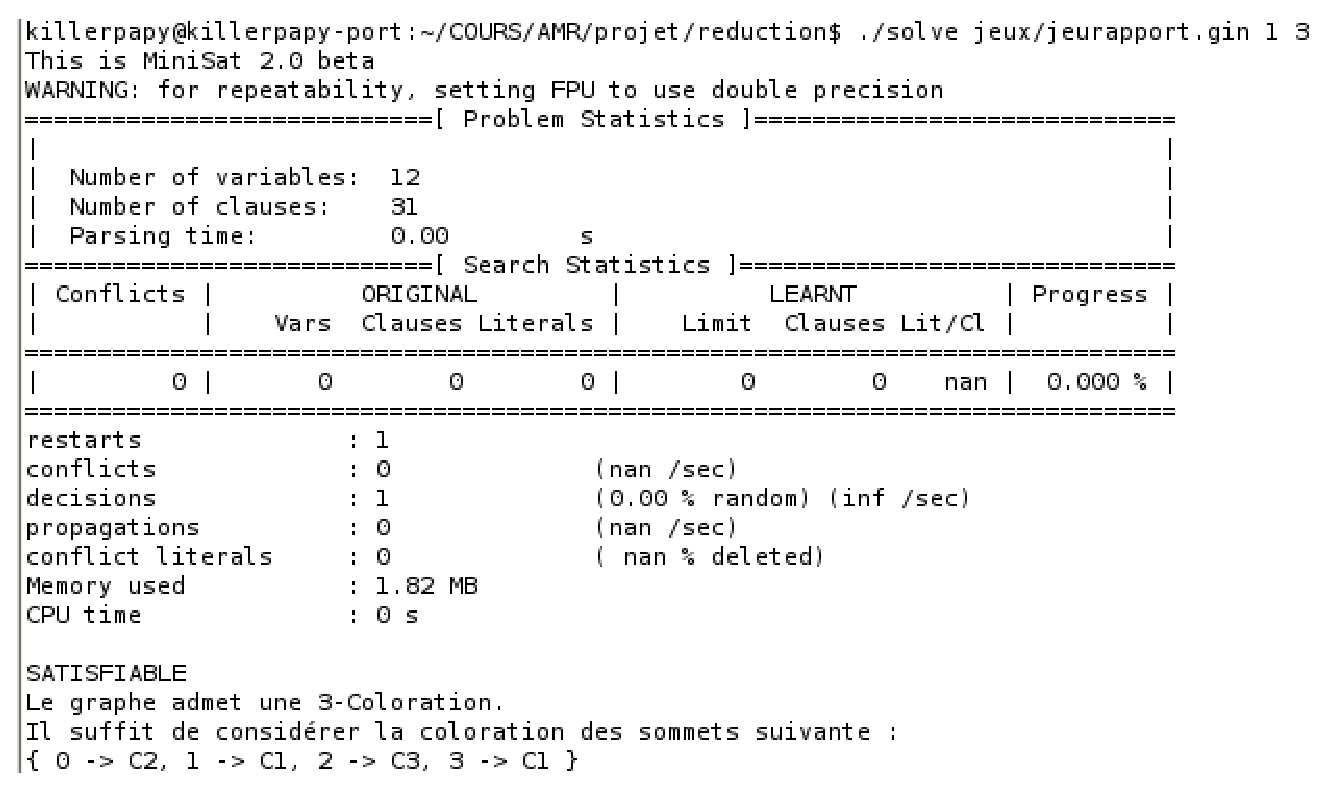
\includegraphics[width=12cm]{images/3-Col.eps}
    \caption{Test de 3-Col sur le graphe \ref{graphe}}
   \end{center}
  \end{figure}
  
  Ce qui donne comme résultat pour \emph{3-Col}: fig.\ref{result} page
  \pageref{result}
  \begin{figure}[!ht]
   \begin{center}
    \includegraphics[height=6cm]{images/jeurapport.ps}
    \caption{Test de 3-Col sur le graphe \ref{graphe} \label{result}}
   \end{center}
  \end{figure}

  \newpage

  \subsection{Circuit Hamiltonien - Cas dangereux\label{an_warningCH}}
  Cas dangereux de graphe qui n'admet pas de \emph{Circuit Hamiltonien}
  (fig.\ref{warningCH} page \pageref{warningCH}).
  \begin{figure}[!ht]
   \begin{center}
    \includegraphics[height=8cm]{images/warningCH.eps}
    \caption{Graphe dangereux pour \emph{Circuit
    Hamiltonien}\label{warningCH}}
   \end{center}
  \end{figure}



